% !TeX root = main.tex 
%!TEX root = main.tex

\newcommand{\bLstar}{\bL^{\star}}
\newcommand{\bRstar}{\bR^{\star}}


\section{Introduction}\label{sec:intro} 

In the semi-streaming model for graph problems, formalized by~\cite{FeigenbaumKMSZ05}, we have an $n$-vertex graph $G=(V,E)$ whose edges are given
to the algorithm in some arbitrarily ordered stream; the algorithm makes one or a few passes over the stream, uses $\Ot(n):= O(n \cdot \poly\!\log{(n)})$ memory, and at the end of the stream, 
outputs a solution to the problem at hand. In this paper, we study \textbf{single-pass} semi-streaming algorithms for the \textbf{maximum matching} problem. 

Alongside the introduction of the model,~\cite{FeigenbaumKMSZ05} observed a simple $(1/2)$-approximation for this problem: greedily maintain a maximal matching of the arriving edges. 
The two decades since then have witnessed a high throughput of results on the semi-streaming matching problem, and yet, this simple algorithm remains the state of the art. A handful of 
impossibility results have also been proven over the years, ruling out approximation ratios of $(2/3)$~\cite{GoelKK12}, $(1-1/e) \sim 0.632$~\cite{Kapralov13}, $(1+\ln{(2)})^{-1} \sim 0.590$~\cite{Kapralov21}, 
and most recently $(8-2\sqrt{10})/3 \sim 0.558$~\cite{AssadiJX26}. 

In light of this state of affairs, whether the half-approximation of the greedy algorithm can be improved has been an outstanding open question since the introduction of the model~\cite{FeigenbaumKMSZ05,KonradMM12,sublinear_open_60,McGregor14,KaleT17,KonradN21}. 
Over the years, this question has been commonly referred to as ``major''~\cite{Tirodkar18,GamlathKMS19,GargKRS20,FischerMU22}, ``central''~\cite{AssadiBKL23,DerakhshanGR25}, ``key''~\cite{AlexandruDKN23}, ``main''~\cite{Bernstein24}, one of the ``most longstanding''~\cite{Behnezhad21,AssadiB21,DerakhshanGR25} or ``most appealing''~\cite{EsfandiariHM16,CormodeJMM17}, ``perhaps the most well-known''~\cite{Gamlath21}, and ``the most basic''~\cite{FeldmanS22} of open questions in the area. It has also been more affectionally called ``vexing''~\cite{ChakrabartiK14},``baffling''~\cite{KaleT17}, ``most tantalizing''~\cite{Wajc21}, ``notorious''~\cite{FeldmanNSZ22}, and ``elusive''~\cite{naidu2024streaming}, among others.  


We fully resolve this question in our work. 

\begin{Theorem}\label{thm:main}
	There is no single-pass semi-streaming algorithm for the maximum bipartite matching problem that can achieve any constant approximation ratio strictly better than half with constant probability. 
\end{Theorem}

\Cref{thm:main} settles the complexity of the semi-streaming matching problem: after all, the naive greedy algorithm turns out to be optimal for this fundamental problem. 

Our proof of~\Cref{thm:main} is based on the \emph{``blueprint framework''} of the recent work of the authors in~\cite{AssadiJX26}. We describe this framework next and put our result in this context. 


\subsection{Blueprint Framework of~\cite{AssadiJX26}} 

In~\cite{AssadiJX26}, we reduced proving lower bounds for semi-streaming matching to constructing ``constant-size'' (relative to stream length) combinatorial
objects called \emph{blueprints}. We now define blueprints and this framework\footnote{We directly define what~\cite{AssadiJX26} calls a \emph{simple} blueprint as the blueprint itself, 
as it is a lot easier to describe and we do not need the extra power of the more general definition.}
(following~\cite{AssadiJX26}, we use `blackboard bold' letters for blueprint notation). 


\begin{definition}\label{def:blueprint}
    For integers $P,C \geq 1$, we define a \textbf{blueprint} with parameters $P,C$ as any bipartite graph $\bG=(\bL,\bR,\bE)$ such that: 
    \begin{itemize}
    \item Vertices in $\bL$ and $\bR$ are identified by tuples in $[C]^P$; specifically, for any $x \in [C]^P$ we have a vertex $\bL(x) \in \bL$ and a vertex $\bR(x) \in \bR$. 
    \item Edges of $\bG$ are partitioned into $P$ groups:
    $
      \bE = \bEE{1} \sqcup \cdots \sqcup \bEE{P}.
    $
    \end{itemize}
\end{definition}
\Cref{def:blueprint} simply gives the ``skeleton'' of a blueprint; what we really need from a blueprint is to satisfy the following two constraints (see~\Cref{sec:prelim} for a quick review of notation).  

\begin{definition}\label{def:proper-blueprint}
	We say a blueprint $\bG=(\bL,\bR,\bE)$ with parameters $(P,C)$ is \textbf{proper} if it satisfies the following constraints:
    \begin{itemize}
        \item \textnormal{\textbf{Matching constraint:}} The edges in $\bE$ form a single matching in $\bG$. 

        \item \textnormal{\textbf{Ban constraints:}} For any $x,y \in [C]^P$ and vertices $\bL(x)$ and $\bR(y)$ incident on the same edge $\be=(\bL(x),\bR(y)) \in \bEE{p}$ for some $p \in [P]$:
	\begin{quote}
		for any $z \in [C]^{P-p+1}$, at least one of vertices $\bL(x_{<p} \conc z)$ or $\bR(y_{<p} \conc z)$ has no edges in $\bG$; we
		say these two vertices are \textbf{banned together} by the edge $\be$.
	\end{quote}
    \end{itemize}
\end{definition}
See~\Cref{fig:ban} for an example of ban constraints.

\begin{figure}[h!]
\centering

\begin{subfigure}[t]{0.48\textwidth}
\centering
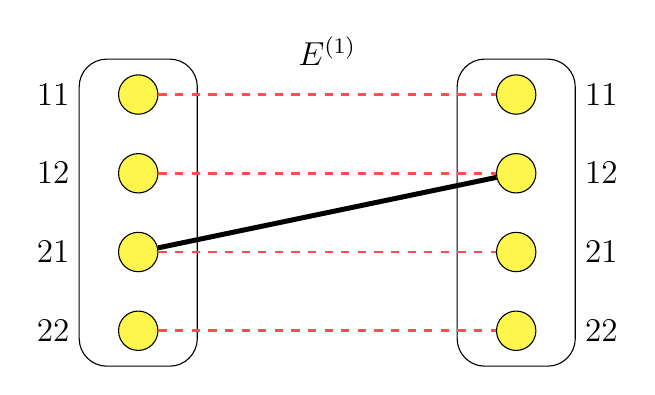
\begin{tikzpicture}[scale=1, every node/.style={font=\large}]
    % styles
    \tikzstyle{vtx}=[circle, draw=black, fill=yellow!70, minimum size=5mm, inner sep=0pt]
    \tikzstyle{dashededge}=[red!70, dashed, line width=1.0pt]
    \tikzstyle{solidedge}=[black, line width=1.8pt]

    % coordinates
    \def\lx{0}
    \def\rx{4.8}
    \def\yA{3}
    \def\yB{2}
    \def\yC{1}
    \def\yD{0}

    % enclosing boxes
    \draw[rounded corners=10pt] (-0.75,-0.45) rectangle (0.75,3.45);
    \draw[rounded corners=10pt] (4.05,-0.45) rectangle (5.55,3.45);

    % left vertices
    \node[vtx] (L11) at (\lx,\yA) {};
    \node[vtx] (L12) at (\lx,\yB) {};
    \node[vtx] (L21) at (\lx,\yC) {};
    \node[vtx] (L22) at (\lx,\yD) {};

    % right vertices
    \node[vtx] (R11) at (\rx,\yA) {};
    \node[vtx] (R12) at (\rx,\yB) {};
    \node[vtx] (R21) at (\rx,\yC) {};
    \node[vtx] (R22) at (\rx,\yD) {};

    % labels
   % labels: placed 0pt away from the enclosing boxes
    \node[anchor=east] at ([xshift=0pt]-0.75,\yA) {$11$};
    \node[anchor=east] at ([xshift=0pt]-0.75,\yB) {$12$};
    \node[anchor=east] at ([xshift=0pt]-0.75,\yC) {$21$};
    \node[anchor=east] at ([xshift=0pt]-0.75,\yD) {$22$};

    \node[anchor=west] at ([xshift=0pt]5.55,\yA) {$11$};
    \node[anchor=west] at ([xshift=0pt]5.55,\yB) {$12$};
    \node[anchor=west] at ([xshift=0pt]5.55,\yC) {$21$};
    \node[anchor=west] at ([xshift=0pt]5.55,\yD) {$22$};

    % title
    \node at (2.4,3.55) {$\mathbb{E}^{(1)}$};

    % dashed edges
    \draw[dashededge] (L11) -- (R11);
    \draw[dashededge] (L12) -- (R12);
    \draw[dashededge] (L21) -- (R21);
    \draw[dashededge] (L22) -- (R22);

    % solid edge
    \draw[solidedge] (L21) -- (R12);
\end{tikzpicture}
\caption{Adding any edge in $\bEE{1}$ bans the pairs in the identity permutation in the entire blueprint.}
\end{subfigure}
\hfill
\begin{subfigure}[t]{0.48\textwidth}
\centering
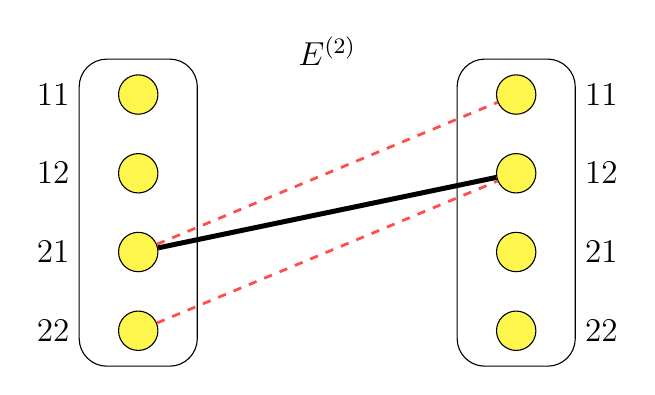
\begin{tikzpicture}[scale=1, every node/.style={font=\large}]
    % styles
    \tikzstyle{vtx}=[circle, draw=black, fill=yellow!70, minimum size=5mm, inner sep=0pt]
    \tikzstyle{dashededge}=[red!70, dashed, line width=1.0pt]
    \tikzstyle{solidedge}=[black, line width=1.8pt]

    % coordinates
    \def\lx{0}
    \def\rx{4.8}
    \def\yA{3}
    \def\yB{2}
    \def\yC{1}
    \def\yD{0}

    % enclosing boxes
    \draw[rounded corners=10pt] (-0.75,-0.45) rectangle (0.75,3.45);
    \draw[rounded corners=10pt] (4.05,-0.45) rectangle (5.55,3.45);

    % left vertices
    \node[vtx] (L11) at (\lx,\yA) {};
    \node[vtx] (L12) at (\lx,\yB) {};
    \node[vtx] (L21) at (\lx,\yC) {};
    \node[vtx] (L22) at (\lx,\yD) {};

    % right vertices
    \node[vtx] (R11) at (\rx,\yA) {};
    \node[vtx] (R12) at (\rx,\yB) {};
    \node[vtx] (R21) at (\rx,\yC) {};
    \node[vtx] (R22) at (\rx,\yD) {};

    % labels
   % labels: placed 0pt away from the enclosing boxes
    \node[anchor=east] at ([xshift=0pt]-0.75,\yA) {$11$};
    \node[anchor=east] at ([xshift=0pt]-0.75,\yB) {$12$};
    \node[anchor=east] at ([xshift=0pt]-0.75,\yC) {$21$};
    \node[anchor=east] at ([xshift=0pt]-0.75,\yD) {$22$};

    \node[anchor=west] at ([xshift=0pt]5.55,\yA) {$11$};
    \node[anchor=west] at ([xshift=0pt]5.55,\yB) {$12$};
    \node[anchor=west] at ([xshift=0pt]5.55,\yC) {$21$};
    \node[anchor=west] at ([xshift=0pt]5.55,\yD) {$22$};

    % title
    \node at (2.4,3.55) {$\mathbb{E}^{(2)}$};

    % dashed edges
    \draw[dashededge] (L21) -- (R11);
    \draw[dashededge] (L22) -- (R12);

    % solid edge
    \draw[solidedge] (L21) -- (R12);
\end{tikzpicture}
\caption{If the same edge was instead added to $\bEE{2}$, it would ban fewer but different pairs.}
\end{subfigure}

\caption{An illustration of ban constraints in a blueprint with $P=C=2$ with labels of vertices drawn next to them. Solid (black) edges show two possible edges in two different blueprints and dashed (red) edges show banned pairs resulting
from inclusion of each of these edges separately.}
\label{fig:ban}
\end{figure}

Finally, the following quantity determines how ``good'' a blueprint is for our purpose.
\begin{definition}\label{def:blueprint-value-approx}
	Define the \textnormal{\textbf{value}} of a blueprint $\bG = (\bL,\bR,\bE)$ as:
 	 \[
    		value(\bG) := \frac{\card{\bE}}{\card{\bL}} = \frac{\card{\bE}}{\card{\bR}} = \frac{\card{\bE}}{C^P}. 
    	\]
\end{definition}

We refer the reader to~\cite{AssadiJX26} for several examples of blueprints and the intuition (and the formal proof) behind the connection between blueprints and semi-streaming matching. For us, we need the following 
theorem that captures the blueprint framework put forward in~\cite{AssadiJX26}\footnote{In light of what we said earlier about \emph{simple} blueprints in~\cite{AssadiJX26}, it is worth 
emphasizing that~\cite{AssadiJX26} proves this theorem for simple blueprints and then shows simple and not-simple blueprints are equivalent; given our construction is already a simple blueprint, we 
do not need this equivalence and defined simple blueprints as blueprints.}.

\begin{theorem}[\!\!{\cite{AssadiJX26}}]\label{thm:framework}
	Suppose there is a proper blueprint $\bG$ and define $\alpha := \frac{2-2 \cdot value(\bG)}{2-value(\bG)}$. 
	Then, for any fixed $\delta > 0$, and any sufficiently large $n$, as a function of $\bG$ and $\delta$, the following holds. 
	Any single-pass semi-streaming algorithm for maximum bipartite matching on $n$-vertex graphs cannot achieve
	an $(\alpha+\delta)$-approximation with probability more than $1-\delta$. 
\end{theorem}

In~\cite{AssadiJX26}, we constructed blueprints with values converging to $(5-\sqrt{10})/3$ which, plugged in~\Cref{thm:framework}, proves the impossibility of better than $(8-2\sqrt{10})/3 \sim 0.558$ approximation
for the semi-streaming matching problem. The limit of the framework of~\cite{AssadiJX26} however is determined by the following quantity
\begin{align}
\sup\set{value(\bG):\text{$\bG$ a proper blueprint}},  \label{eq:sup}
\end{align}
which was not well understood in~\cite{AssadiJX26}. 

\paragraph{Our blueprint construction.} 
We determine the optimal value of~\Cref{eq:sup} in this work, proving the following, which is the main \emph{technical} result of our work. 
\begin{theorem}\label{thm:blueprint}
	There is a sequence of proper blueprints $(\bG_m)_{m \geq 1}$ with parameter $P_m \to \infty$ and 
	\[
		\lim_{m \to \infty} value(\bG_m) = 2/3.
	\] 
\end{theorem}

Plugging in the blueprints in~\Cref{thm:blueprint} in~\Cref{thm:framework} then immediately proves~\Cref{thm:main}. Our proof of~\Cref{thm:blueprint} is  constructive and we 
give an explicit description of the blueprints in the family (even though this is not required to apply~\Cref{thm:framework}). We also note that as pointed out in~\cite{AssadiJX26}, 
one does need $P \to \infty$ for the value of the blueprint to be able to reach $2/3$. 


As an aside, we should note that, technically speaking, one also needs to prove an upper bound on~\Cref{eq:sup} to fully determine the value of~\Cref{eq:sup} (although this is not needed for proving~\Cref{thm:main}). However, a $2/3$ upper bound follows 
immediately from~\Cref{thm:framework} and the greedy algorithm for the semi-streaming matching problem. We give a different and direct proof of this upper bound in~\Cref{app:2-3-upper} as it provides further insight into the structure of blueprints. 


\subsection{Our Blueprint Construction at a High Level}\label{sec:ideas} 

Blueprints in~\Cref{thm:blueprint} are created by using elementary properties of random walks on the integer line. The general idea of the construction is as follows (as our blueprints 
are \emph{entirely disjoint} from~\cite{AssadiJX26} technique-wise, we will not review those blueprints and refer the reader to~\cite{AssadiJX26}). 

\paragraph{Vertices and random walks.} Let $m \geq 1$ be an integer and $\bG = (\bL,\bR,\bE)$ be a blueprint with parameters $P$ and $C$ that depend on $m$. 
To any label $x \in [C]^P$, we assign a walk $W(x)$ on $\set{0,\ldots,2m}$ that starts from some state in $[2m-1]$ and in each step moves to either a one larger or one smaller 
state and terminates when it reaches $0$ or $2m$. Define the \emph{reflection} walk $\barW(x)$ that starts at the same state as $W(x)$ but in every step, takes the opposite direction as $W(x)$. 
This assignment is done so that for $x$ chosen uniformly from $[C]^P$, $W(x)$ (also $\barW(x)$) becomes a random walk whose starting state is sampled from some distribution $\mu$ and 
each of its step is chosen uniformly. This is done by using the first index of $[P]$ 
to simulate sampling from $\mu$ (by partitioning $[C]$ into intervals of lengths proportional to $\mu(i)$-values) and remaining indices to simulate the random walk (by partitioning $[C]$ into two equal halves); see~\Cref{fig:W(x)} for a quick illustration (we have
skipped one other coordinate in $[P]$ called ``delay'' and will explain it later). 

\paragraph{Edges between $0$-reaching random walks.} Let $\bLstar$ (resp. $\bRstar$) be vertices $\bL(x)$ (resp. $\bR(x)$) whose random walk $W(x)$ (resp. $\barW(x)$) reaches $0$. Moreover, for any $j \in [2m-1]$ and time $t \in [P-1]$, let $\bLstar_{j,t}$ denote the following subset of $\bLstar$: 
\begin{itemize}
	\item All $\bL(x) \in \bL$ such that $W(x)$ reaches $0$, $W(x)$ has $j$ as the \emph{maximum} state it ever visits, and, it has visited $j$ for the \emph{first} time at the $t$-th step of the walk. 
\end{itemize} 
We define $\bRstar_{j,t}$ analogously using the reflection walk $\barW$. In the blueprint, we add a \emph{matching} between $\bLstar_{j,t}$ and $\bRstar_{2m-j,t}$ in $\bEE{t+1}$ with size equal to the smaller of the two. 

\paragraph{Properness of the blueprint.} We need to ensure the inserted edges form a matching and that the ban constraints are satisfied. The former is easy to verify as $\bLstar_{j,t},\bRstar_{j,t}$ sets are disjoint for different $j,t$ and each is incident on a matching. We now prove the ban constraint.

Consider any edge between $\bL(x) \in \bLstar_{j,t}$ and $\bR(y) \in \bRstar_{2m-j,t}$ in some $\bEE{t+1}$ for $j \in [2m-1]$ and $t \in [P-1]$ (all edges are of this form). The ban constraint requires that for any $z \in [C]^{P-t}$, at most one of $\bL(x_{\leq t} \circ z)$ or $\bR(y_{\leq t} \circ z)$ is matched. Fixing $x_{\leq t}$ and $y_{\leq t}$ ``brings'' any walk of $W(x_{\leq t} \circ z)$ and $\barW(y_{\leq t} \circ z)$ 
to the states $j$ and $2m-j$ at their $t$-th step (by the definitions of $\bLstar_{j,t},\bRstar_{2m-j,t}$). Now, suppose $\bL(x_{\leq t} \circ z)$ is matched. Then, it means that the remainder of the walk, which with a slight abuse of notation we denote by $W(z)$, 
will move from the state $j$, uses $z$, and reaches $0$ (so $\bL(x_{\leq t} \circ z)$ becomes matched). But then, the reflection walk $\barW(z)$ will move in the ``opposite'' direction: it moves from $2m-j$, uses $z$, and thus reaches $2m$ instead; this means 
that $\bR(y_{\leq t} \circ z)$ will not be matched, as desired. This is the entire proof of the ban constraint (see also~\Cref{fig:W}). 

\paragraph{Value calculation.} The final step is to consider the value of this blueprint. In our construction, we are going to ensure that the sizes of each of $\bLstar_{j,t}$ and $\bRstar_{2m-j,t}$ that are matched together are 
(almost) equal to each other. This will ensure that the size of the matching of the blueprint is (almost) $\card{\bLstar}$, which implies that
\begin{align}
	value(\bG) := \frac{\card{\bLstar}}{C^P} = \Pr_{x \in_R [C]^P}\paren{\text{walk $W(x)$ reaches $0$}}.  \label{eq:over-value}
\end{align}
As stated earlier, the constraint we have is that $\bLstar_{j,t}$ and $\bRstar_{2m-j,t}$ sets should have roughly the same size. For now let us \emph{relax} this constraint to instead 
ask that $\bLstar_{j} := \cup_t~ \bLstar_{j,t}$ and $\bRstar_{2m-j} := \cup_t~ \bRstar_{2m-j,t}$ have the same size. This translates to having, 
\begin{align}
	&\forall j \in [2m-1] \Pr_{x \in_R [C]^P}\paren{\text{walk $W(x)$ reaches $0$ and maximum state it visits is $j$}} \notag \\
	&\hspace{90pt}= \Pr_{x \in_R [C]^P}\paren{\text{walk $\barW(x)$ reaches $0$ and maximum state it visits is $2m-j$}}. \label{eq:over-constraint}
\end{align}
The underlying distributions of both $W(x)$ and $\barW(x)$ here are just standard random walks starting from a random state chosen according to 
some distribution $\mu$. Thus, at this point, the goal is to maximize~\Cref{eq:over-value} subject to the constraints in~\Cref{eq:over-constraint}, by choosing
the initial distribution $\mu$ carefully. 

The type of random walk we have here is often called ``gambler's ruin'' and is well studied as one of the simplest examples of Markov Chains; see, e.g.~\cite[Section 2.1]{levin2026markov}. 
For instance, it is known that starting from a \emph{uniform} distribution $\mu$, maximum visited state will also be distributed uniformly and thus certainly satisfies~\Cref{eq:over-constraint}. But in this case, 
the walk has an equal chance of reaching $0$ and $2m$, making $value(\bG)=1/2$ only. However, by ``shifting'' the distribution of $\mu$ towards $0$, while still enforcing~\Cref{eq:over-constraint}, one
can improve the objective function. We are not aware of prior work that study this particular formulation but solving this optimization problem has a standard method: one can cast the problem as a 
linear program in $\mu(i)$-values and obtain a closed form formula for the variables. Doing this in our case leads to the objective value of $2m/(3m+1)$ (see~\Cref{lem:start-state}), giving us 
the desired value for the blueprint. 

There is however one catch with the argument above: we moved from enforcing (almost) equality in sizes of $\bLstar_{j,t}$ and $\bRstar_{2m-j,t}$ to only $\bLstar_j$ and $\bRstar_{2m-j}$; but, symmetrizing the distribution 
of maxima (through the choice of $\mu$) does not mean the time to reaching them will also be symmetric. This however can be handled rather easily by introducing \textbf{random delays} in the random walks: we dedicate one more coordinate in $[P]$
for this task, and start the random walks at different time stages to ensure that distribution of ``time to hit maximum'' becomes (almost) uniform over the time steps which fixes the above problem. 

\subsection{Further Corollaries of Our Result}\label{sec:corollary} 

We mention two further corollaries of our results. The first one is for the matching problem but in another model, the \emph{online matching with preemption}, whereas the second one is for another problem, the \emph{minimum vertex cover}, but back
in the semi-streaming model. 

\paragraph{Online matching with preemption.} In this problem, the edges of the graph are arriving sequentially
and the algorithm must maintain a matching by accepting or rejecting arriving edges and can preempt previously accepted ones by discarding them. This model is a generalization of the original online matching (with one-sided vertex arrival) in~\cite{KarpVV90}. 

The \emph{competitive ratio} of an algorithm in this model is the ratio of the matching size provided by the algorithm compared to the maximum matching of the graph. 
The greedy algorithm achieves a half competitive ratio in this model with no need for preemption. When preemptions are not allowed,~\cite{GamlathKMSW19} proved that  
half approximation is optimal. No better algorithm is known even when preemption is allowed and a series of results over the years have ruled out competitive ratios of 
$(1-1/e) \sim 0.632$~\cite{KarpVV90}, $(1+\ln{(2)})^{-1} \sim 0.590$~\cite{EpsteinLSW13}, $(2-\sqrt{2}) \sim 0.585$~\cite{HuangPTTWZ19}, and very recently $0.5661$~\cite{KissS26}\footnote{It is not a coincidence 
that these numbers and their progressions sound very similar to the ones mentioned for the semi-streaming matching: until~\cite{AssadiJX26}, all previous semi-streaming matching lower bounds in~\cite{GoelKK12,Kapralov13,Kapralov21} 
were based on generalizing online preemptive matching instances to the semi-streaming model (but using completely white-box arguments); see~\cite{Kapralov21} for a detailed discussion of this topic.}.
We prove that the greedy algorithm is also optimal for this problem. 

\begin{corollary}\label{cor:online}
	There is no algorithm for the online matching problem with preemption with an expected competitive ratio 
	strictly better than half by any constant. 
\end{corollary}

As already observed in~\cite{AssadiJX26}, the blueprint framework also implies lower bounds for the online matching problem with preemption (given this connection, technically, the best known bound on the competitive ratios 
prior to our work is the $0.558$ bound of~\cite{AssadiJX26}, which was obtained independently and concurrently to~\cite{KissS26}). Thus,~\Cref{cor:online} directly follows from our~\Cref{thm:blueprint} and the 
blueprint framework of~\cite{AssadiJX26}. 



\paragraph{Semi-streaming (bipartite) vertex cover.} Going back to the semi-streaming model, a closely related problem to maximum bipartite matching is its dual, the minimum bipartite vertex cover problem. 
The greedy algorithm is also a $2$-approximation algorithm for this problem and no better algorithms are known. It has been asked in prior work, e.g.,~\cite{AssadiBBMS19,DerakhshanGR25} whether this algorithm can be improved. 
We resolve this question in this work. 

\begin{corollary}\label{cor:vc}
	There is no single-pass semi-streaming algorithm for the minimum bipartite vertex cover problem that can achieve any constant approximation ratio strictly better than two with constant probability. 
\end{corollary}
We note that prior to our work, no $2$-approximation lower bounds were known for this problem even in general graphs (the UGC hardness of $2$-approximation vertex cover~\cite{KhotR03} does not imply a semi-streaming lower bound, 
as runtime of algorithms is not bounded in this model). 

The proof of this result is again by observing that the blueprint framework of~\cite{AssadiJX26} also implies lower bounds for the vertex cover problem given the duality of the problems (plus a standard modification for 
going from matching lower bounds to vertex cover ones as done previously in the literature, e.g., in~\cite{AssadiK17,DerakhshanGR25}). 



